\chapter{Embryonale ontwikkeling van gewervelden}\label{ch:b2:vertebrate-development}

Een kikkerei is een bolletje van twee millimeter doorsnede, donker aan de
bovenkant en licht aan de onderkant. Binnen een dag heeft het zich in
duizenden cellen gedeeld; binnen twee dagen is een laag van die cellen
via een groef naar binnen gerold om een darm te maken en een staaf langs de
rug aan te leggen; binnen drie dagen heeft de laag boven die staaf zich
opgevouwen tot een buis die de hersenen en het ruggenmerg zal worden. Er
is niets toegevoegd behalve water. De informatie die van één cel een
zwemmend kikkervisje maakt, zat in het ei en zijn genoom, en de manier
waarop ze zich ontvouwt --- \omterm{def:b2:vertebrate-development:egg}{klieving}, gastrulatie, neurulatie, de inductie
van elk deel door zijn buren --- is herkenbaar dezelfde bij een vis, een
kuiken en een muis. Dit hoofdstuk volgt een embryo van een gewervelde door
die stappen en beschrijft de experimenten die lieten zien hoe elk deel
ervan te horen krijgt wat het moet worden.

\section{Van ei tot blastula}

\begin{definition}[Het ei en zijn assen]\label{def:b2:vertebrate-development:egg}
\index{animale pool}\index{vegetatieve pool}\index{dooier}\index{klieving}
Een ei van een gewervelde is al vóór de bevruchting gepolariseerd: de
\emph{animale pool} bevat de kern en het meeste cytoplasma, de
\emph{vegetatieve pool} de \emph{dooier}, de voorraad eiwit en lipide
waarvan het embryo zal leven tot het zich voedt. De hoeveelheid dooier
bepaalt het patroon van alles wat volgt: een ei van een zee-egel of een
zoogdier heeft er vrijwel geen en klieft volledig in gelijke cellen; een
kikkerei heeft een matige hoeveelheid en klieft volledig maar ongelijk
(kleine cellen boven, grote dooierrijke cellen onder); een ei van een vis
of een vogel bestaat bijna helemaal uit dooier en klieft alleen in een
schijfje cytoplasma daarbovenop. Bij de kikker legt het punt waar de
zaadcel binnenkomt de tweede as vast: de cortex draait dertig graden van
dat punt weg en legt tegenover het binnenkomstpunt een \emph{grijze
halvemaan} bloot, en die kant wordt de rug. \emph{Klieving} is een reeks
snelle mitosen zonder groei --- de cellen halveren bij elke deling in
grootte ---, aangedreven door maternale mRNA's en eiwitten die in het ei
zijn opgeslagen, terwijl de eigen genen van het embryo stil blijven tot de
\emph{midblastulatransitie}, zo'n twaalf delingen verder.
\end{definition}

\begin{omfigure}
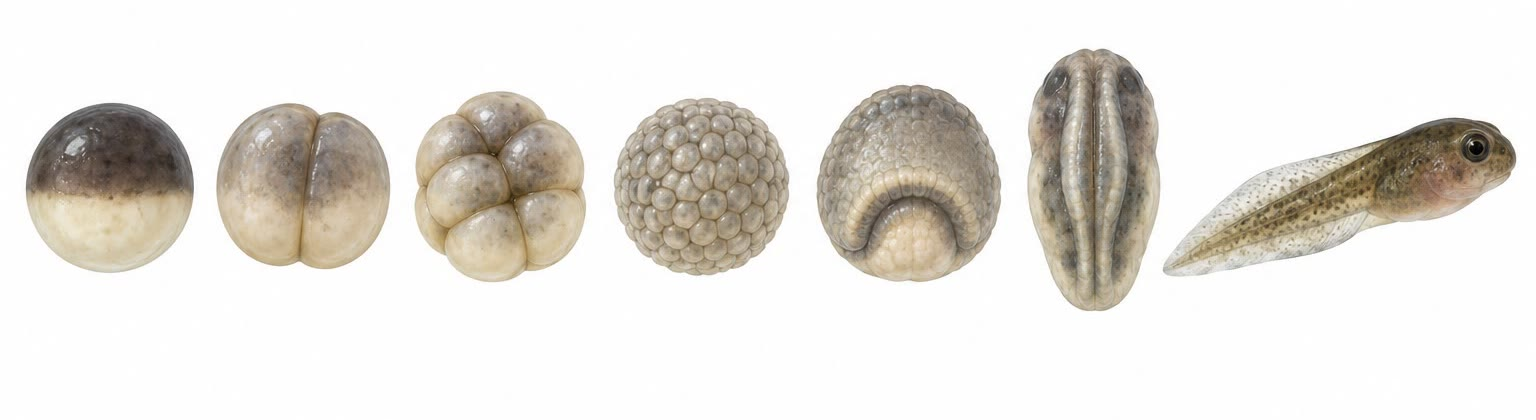
\includegraphics[width=0.9\linewidth]{images/book4/ai/b4-10-frog-development.jpg}

{\small De ontwikkeling van een kikker vanaf het bevruchte ei: \omterm{def:b2:vertebrate-development:egg}{klieving} tot
een \omterm{def:b2:vertebrate-development:blastula}{blastula}, gastrulatie, de neurula met haar neurale plooien, en het
kikkervisje --- alles in enkele dagen, zonder groei.}
\end{omfigure}

\begin{theorem}[De rekenkunde van de klieving]\label{thm:b2:vertebrate-development:cleavage}
Na $k$ synchrone \omterm{def:b2:vertebrate-development:egg}{klievingen} bestaat een ei met volume $V_0$ uit $2^{k}$
cellen met gemiddeld volume $V_0/2^{k}$ en straal $r_0/2^{k/3}$, en is het
totale oppervlak met $2^{k/3}$ gegroeid; de verhouding van kern- tot
cytoplasmavolume, die in een kikkerei rond $10^{-4}$ begint, stijgt
met $2^{k}$ en bereikt na ongeveer tien delingen die van een gewone cel
($\sim 0.1$). Het is deze stijgende verhouding --- de titratie van een
vaste maternale voorraad van een of andere remmer door een exponentieel
groeiende hoeveelheid DNA --- die de midblastulatransitie in gang zet: de
delingen vertragen, worden asynchroon, en het zygotische genoom schakelt
aan.
\end{theorem}
\begin{proof}
Het volume blijft bij \omterm{def:b2:vertebrate-development:egg}{klieving} behouden, dus heeft elk van de $2^{k}$
cellen $V_0
2^{-k}$ en, als bol, een straal $r_0 2^{-k/3}$; hun totale oppervlak is
$2^{k}\cdot 4\pi r_0^{2}\, 2^{-2k/3} = 4\pi r_0^{2}\, 2^{k/3}$. Elke
cel behoudt één kern van vaste grootte, zodat de verhouding schaalt als
$2^{k}$ vanaf $10^{-4}$: $2^{10} = 1024$ brengt haar op $0.1$. De
transitie van de kikker valt bij de twaalfde deling, in overeenstemming
met een drempel die iets later wordt bereikt.
\end{proof}
\begin{proof}[Bewijsmateriaal]
Newport en Kirschner (1982) voegden extra DNA toe aan kikkereieren en
vonden dat de transitie zoveel delingen eerder kwam als het DNA in overmaat
was; cytoplasma verwijderen had hetzelfde effect. De klok is geen tijd of
een telling van delingen, maar een verhouding.
\end{proof}

\begin{definition}[Blastula]\label{def:b2:vertebrate-development:blastula}
\index{blastula}\index{blastocoel}
De \omterm{def:b2:vertebrate-development:egg}{klieving} eindigt in een \emph{blastula}: een holle bol (kikker,
zee-egel) of een schijf (vis, vogel) van enkele duizenden cellen rond een
holte, het \emph{blastocoel}. Zijn cellen zien er nog ongespecialiseerd
uit, maar ze zijn niet gelijkwaardig: een \emph{lotkaart}, gemaakt door
plekjes van het oppervlak met kleurstoffen te merken en ze te volgen, laat
zien dat het animale kapje huid en zenuwstelsel zal geven
(\emph{ectoderm}), de equatoriale gordel spieren, skelet, nieren en bloed
(\emph{mesoderm}), en de vegetatieve massa de darm en zijn organen
(\emph{endoderm}). Deze drie \emph{kiembladen} zijn bij elke gewervelde
dezelfde, en de volgende stap is ze op hun plaats te brengen: het mesoderm
en het endoderm liggen buiten en moeten naar binnen.
\end{definition}

\section{Gastrulatie en neurulatie}

\begin{proposition}[Gastrulatie]\label{prop:b2:vertebrate-development:gastrulation}
\index{gastrulatie}\index{blastoporus}\index{oerdarm}\index{chorda}
\emph{Gastrulatie} is het geheel van celbewegingen dat de eenlagige
\omterm{def:b2:vertebrate-development:blastula}{blastula} omvormt tot een drielagige \emph{gastrula}. Bij de kikker begint
ze onder de grijze halvemaan: de cellen daar veranderen van vorm, trekken
hun buitenste uiteinden samen tot flessen, en het oppervlak plooit in tot
een groef, de \emph{blastoporus}. Daardoor stromen mesoderm en endoderm naar
binnen (\emph{involutie}), rollen over de lip en bewegen naar voren langs het
dak van de holte; het animale kapje spreidt zich naar beneden uit om de
buitenkant te bedekken (\emph{epibolie}); de blastoporus sluit zich tot een
ring rond de laatste dooierrijke cellen. Binnenin is een nieuwe holte,
bekleed met endoderm, de \emph{oerdarm}, de toekomstige darm, en het
mesoderm dat als eerste naar binnen rolde, langs de middellijn, is een
stijve staaf geworden, de \emph{chorda}, de as van elk embryo van een
gewervelde en de structuur die de stam haar naam geeft. Bij vogels en
zoogdieren gebeuren dezelfde bewegingen door een spleet, de
\emph{primitiefstreep}, in een platte schijf; bij vissen spreidt de schijf
zich over de \omterm{def:b2:vertebrate-development:egg}{dooier} uit. De choreografie verschilt met de \omterm{def:b2:vertebrate-development:egg}{dooier}; het
resultaat --- ectoderm buiten, endoderm langs de darm, mesoderm ertussen,
chorda in de middellijn --- is hetzelfde.
\end{proposition}

\begin{omfigure}
\begin{tikzpicture}[every node/.style={font=\scriptsize}, >=stealth]
  % blastula
  \begin{scope}
    \draw[thick, fill=omDef!15] (0,0) circle (1.3);
    \draw[thick, fill=white] (0,0.2) circle (0.75);
    \fill[omExo!40] (0,0) ++(-1.3,0) arc (180:360:1.3 and 1.3) -- cycle;
    \draw[thick] (0,0) circle (1.3);
    \node at (0,0.2) {blastocoel};
    \node[below, align=center] at (0,-1.45) {blastula\\animaal kapje (blauw), dooierrijke cellen (grijs)};
  \end{scope}
  % early gastrula: blastopore forming
  \begin{scope}[xshift=4.2cm]
    \draw[thick, fill=omDef!15] (0,0) circle (1.3);
    \draw[thick, fill=white] (0,0.25) circle (0.7);
    \fill[omExo!40] (0,0) ++(-1.3,0) arc (180:360:1.3 and 1.3) -- cycle;
    \draw[thick] (0,0) circle (1.3);
    \draw[very thick, omThm] (1.0,-0.85) .. controls (0.5,-0.6) and (0.4,-0.3) .. (0.55,0.0);
    \draw[->, thick, omThm] (1.15,-0.7) .. controls (0.6,-0.4) .. (0.4,0.1);
    \draw[omThm] (1.0,-0.85) -- (0.9,-1.25); \node[omThm, anchor=north west] at (0.6,-1.2) {lip van de blastoporus};
    \node[below, align=center] at (0,-1.45) {vroege gastrula\\cellen rollen over de lip};
  \end{scope}
  % late gastrula
  \begin{scope}[xshift=8.4cm]
    \draw[thick, fill=omDef!15] (0,0) circle (1.3);
    \draw[thick, fill=omExo!25] (0,0.05) circle (0.95);
    \draw[thick, fill=white] (0.15,-0.1) ellipse (0.55 and 0.4);
    \draw (0.6,-0.3) -- (1.6,-1.15); \node[anchor=west] at (1.6,-1.15) {oerdarm};
    \draw[very thick, omThm] (-0.9,0.35) .. controls (-0.2,0.6) .. (0.8,0.4);
    \draw[omThm] (0.0,0.48) -- (-0.9,1.55); \node[omThm, anchor=east] at (-0.9,1.55) {chorda};
    \draw[thick] (1.1,-0.7) -- (1.3,-0.5);
    \node[right] at (1.3,-0.5) {blastoporus};
    \node[below, align=center] at (0,-1.45) {late gastrula: drie lagen,\\darmholte, chorda op het dak};
  \end{scope}
\end{tikzpicture}

{\small Gastrulatie bij de kikker, in doorsnede. Cellen rollen over de lip
van de blastoporus naar binnen; het endoderm bekleedt een nieuwe darmholte,
en het eerste mesoderm dat binnenkomt, wordt de chorda langs de middellijn.}
\end{omfigure}

\begin{proposition}[Neurulatie en het bouwplan]\label{prop:b2:vertebrate-development:neurulation}
\index{neurulatie}\index{neurale buis}\index{somiet}\index{neurale lijst}
Het ectoderm boven de chorda verdikt zich tot een \emph{neurale plaat},
waarvan de randen als plooien omhoogkomen en in de middellijn samenkomen
tot de \emph{\omterm{prop:b2:vertebrate-development:neurulation}{neurale buis}}, de toekomstige hersenen en het ruggenmerg, die
onder de huid wegzakt; cellen van de kam van de plooien, de \emph{\omterm{prop:b2:vertebrate-development:neurulation}{neurale
lijst}}, migreren weg en maken de perifere zenuwen, de pigmentcellen, het
bijniermerg en een groot deel van het gezicht. Aan weerszijden van de
chorda segmenteert het mesoderm in blokken, de \emph{somieten}, het ene paar
na het andere van kop tot staart, die de wervels, de rompspieren en de
lederhuid geven; het laterale mesoderm splitst zich in de lagen die de
lichaamsholte bekleden en het hart en de ledematen maken; de endodermbuis
laat de longen, de lever en de alvleesklier uitknoppen. Aan het eind van de
neurulatie heeft het embryo het bouwplan van een gewervelde --- een dorsale
zenuwstreng boven een chorda, een ventrale darm, gesegmenteerde spieren, een
kop --- bij een lengte van enkele millimeters, en de rest van de
ontwikkeling is de uitwerking van organen vanuit dit plan
(\cref{ch:b2:limb-organogenesis}).
\end{proposition}

\begin{omfigure}
\begin{tikzpicture}[every node/.style={font=\scriptsize}]
  \foreach \x/\lab in {0/{neurale plaat}, 4.0/{neurale plooien rijzen op}, 8.0/{neurale buis gesloten; neurale lijst migreert}} {
    \begin{scope}[xshift=\x cm]
      \draw[thick, fill=omExo!25] (-1.6,0) rectangle (1.6,-1.6);
      \draw[thick, omThm, fill=omThm!30] (0,-0.75) circle (0.28);
      \draw[thick, fill=omProp!30] (-1.3,-0.75) circle (0.32); \draw[thick, fill=omProp!30] (1.3,-0.75) circle (0.32);
      \node[below, align=center, text width=3.4cm] at (0,-1.7) {\lab};
    \end{scope}
  }
  \draw[very thick, omDef] (-1.6,0) -- (-0.7,0) .. controls (-0.3,0.15) and (0.3,0.15) .. (0.7,0) -- (1.6,0);
  \draw[very thick, omDef] (2.4,0) -- (3.3,0) .. controls (3.3,0.9) and (3.6,0.1) .. (4.0,0.0) .. controls (4.4,0.1) and (4.7,0.9) .. (4.7,0) -- (5.6,0);
  \draw[very thick, omDef] (6.4,0.05) -- (9.6,0.05);
  \draw[very thick, omDef, fill=omDef!20] (8.0,-0.3) circle (0.3);
  \foreach \p in {(7.35,-0.4),(8.65,-0.4)} \fill[omDef!70!black] \p circle (0.07);
  \node[omThm, anchor=west] at (9.8,-0.75) {chorda};
  \node[omProp, anchor=west] at (9.8,-1.15) {somiet};
  \node[omDef, anchor=west] at (9.8,-0.3) {neurale buis};
  \node[omDef!70!black, anchor=west] at (9.8,0.1) {cellen van de neurale lijst};
\end{tikzpicture}

{\small Neurulatie in dwarsdoorsnede: het ectoderm boven de chorda (rood)
verdikt, plooit en sluit zich tot de \omterm{prop:b2:vertebrate-development:neurulation}{neurale buis} (blauw), terwijl het
mesoderm naast de chorda in somieten (oranje) segmenteert en cellen van de
\omterm{prop:b2:vertebrate-development:neurulation}{neurale lijst} de sluitende plooien verlaten.}
\end{omfigure}

\begin{omfigure}
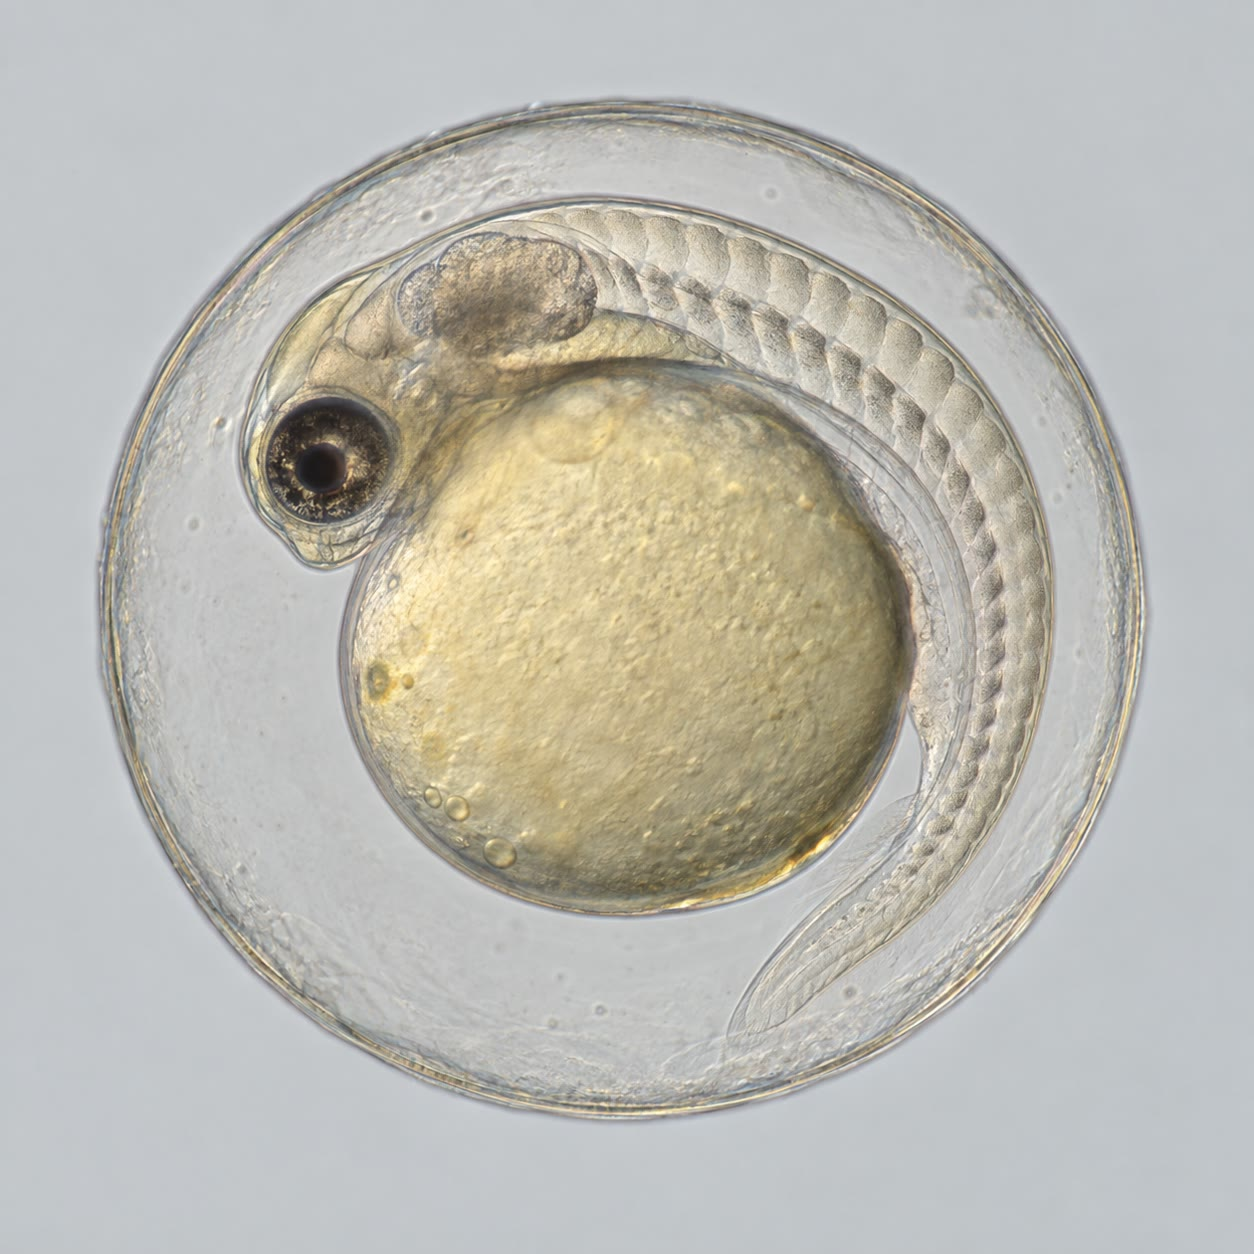
\includegraphics[width=0.42\linewidth]{images/book4/ai/b4-10-zebrafish-embryo.jpg}\hspace{0.04\linewidth}
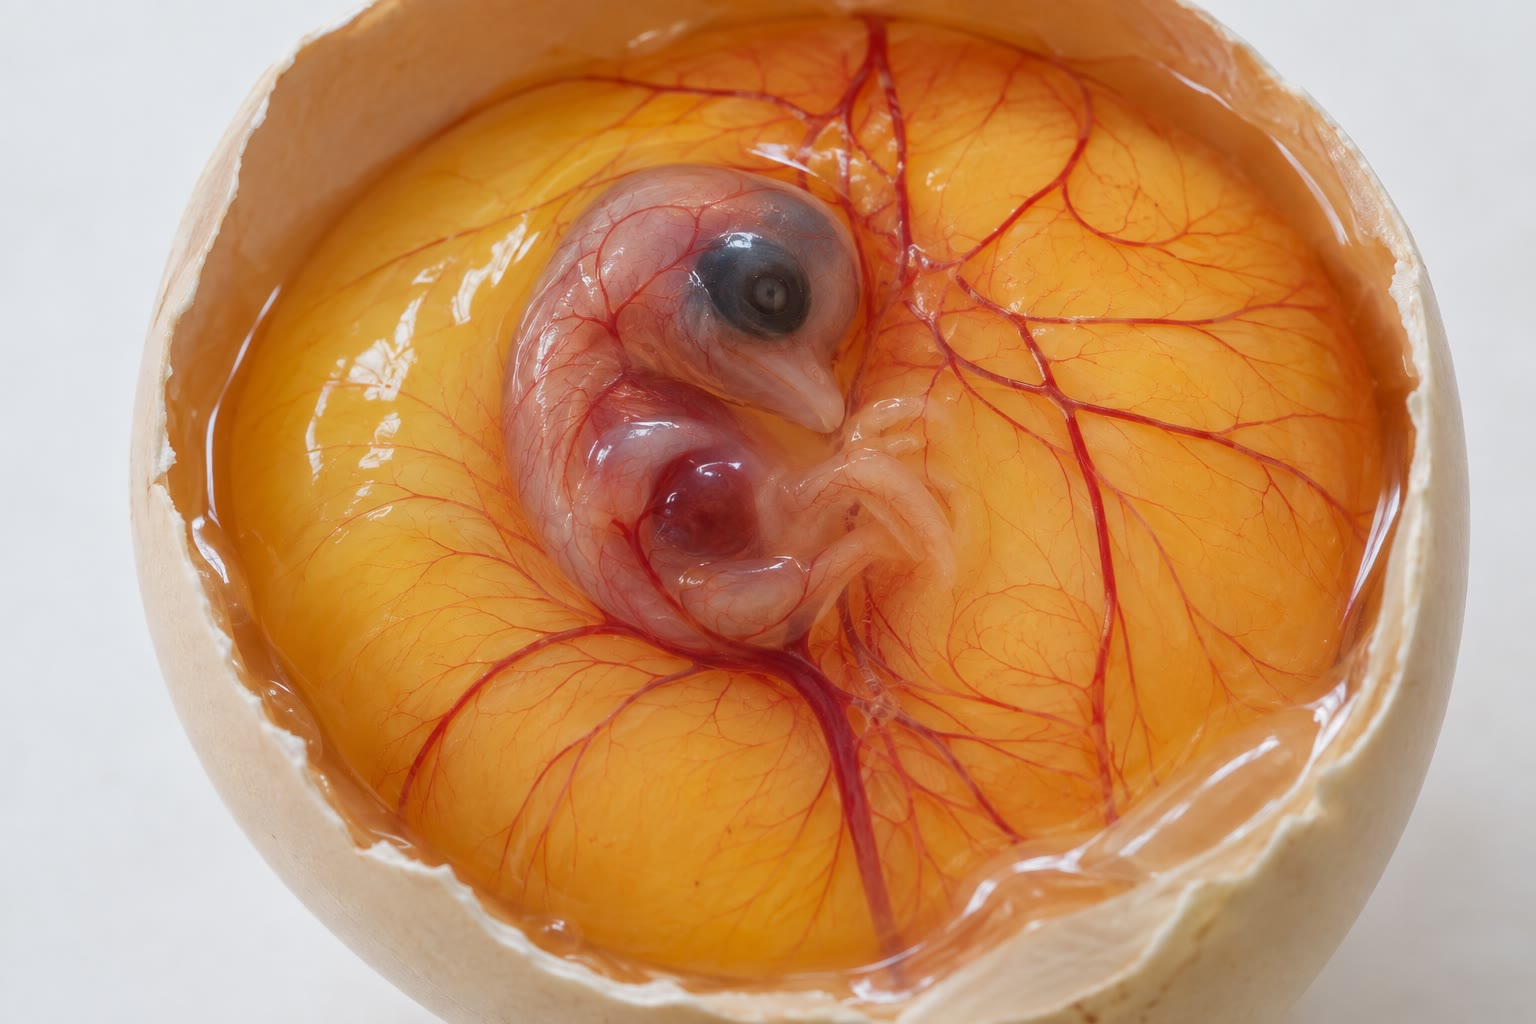
\includegraphics[width=0.5\linewidth]{images/book4/ai/b4-10-chick-embryo.jpg}

{\small Links: een zebravisembryo van één dag oud in zijn chorion,
opgekruld rond zijn \omterm{def:b2:vertebrate-development:egg}{dooier}, met oog, hersenen en een rij somieten.
Rechts: een kuikenembryo van drie dagen op zijn \omterm{def:b2:vertebrate-development:egg}{dooier}, met een hart dat al
klopt en bloedvaten die zich over de \omterm{def:b2:vertebrate-development:egg}{dooier} uitspreiden om het te voeden.}
\end{omfigure}

\section{Inductie: hoe cellen leren waar ze zijn}

\begin{definition}[Inductie en competentie]\label{def:b2:vertebrate-development:induction}
\index{inductie (embryonale)}\index{competentie}\index{organisator}
\emph{Inductie} is het proces waarbij een groep cellen met een signaal het
lot van een naburige groep verandert; de reagerende cellen moeten
\emph{competent} zijn --- in staat te antwoorden, wat ze slechts een
beperkte tijd zijn. De ontwikkeling is een keten van inducties: de
vegetatieve cellen induceren mesoderm in de cellen erboven; het dorsale
mesoderm --- de \emph{organisator} aan de lip van de blastoporus ---
induceert de neurale plaat in het ectoderm erboven en geeft het mesoderm
aan weerszijden een patroon; de chorda induceert de bodem van de \omterm{prop:b2:vertebrate-development:neurulation}{neurale
buis}; het oogblaasje, een uitstulping van de hersenen, induceert een lens in
de huid die het raakt; de lens induceert het hoornvlies. Elk geïnduceerd
weefsel wordt een inductor van het volgende. De signalen behoren tot een
handvol families van uitgescheiden eiwitten die steeds opnieuw worden
gebruikt --- dezelfde die een ledemaat een patroon geven
(\cref{ch:b2:limb-organogenesis}) en die bij de volwassene de signalering
van \cref{ch:b2:cell-signalling} verzorgen.
\end{definition}
\begin{proof}[Bewijsmateriaal]
Spemann en Mangold (1924) sneden de dorsale lip van de blastoporus uit een
vroege gastrula van één soort watersalamander en transplanteerden die naar
de ventrale kant van een andere soort, met een andere pigmentatie, zodat
cellen van gastheer en transplantaat van elkaar te onderscheiden waren. Het
transplantaat werd niet eenvoudig wat het ter plaatse zou zijn geworden:
het rolde naar binnen, vormde chorda, en \emph{induceerde het eigen ventrale
ectoderm van de gastheer} tot het maken van een tweede \omterm{prop:b2:vertebrate-development:neurulation}{neurale buis} en,
daarnaast, somieten van de gastheer --- een volledig tweede embryo,
grotendeels uit cellen van de gastheer, buik aan buik met het eerste
verbonden. Geen enkel ander stuk van de gastrula kon dit. Ze noemden de lip
de \omterm{def:b2:vertebrate-development:induction}{organisator}; zijn signalen (eiwitten die de ventraliserende factor BMP
blokkeren) werden zeventig jaar later geïdentificeerd.
\end{proof}

\begin{omfigure}
\begin{tikzpicture}[every node/.style={font=\scriptsize}, >=stealth]
  % donor
  \draw[thick, fill=omDef!12] (0,0) circle (1.3); \node[above] at (0,1.4) {donorgastrula (licht)};
  \draw[very thick, omThm] (0.85,-0.95) arc (-45:-20:1.3); \node[omThm, right] at (1.2,-0.8) {dorsale lip};
  \draw[->, thick] (1.6,-0.3) -- (3.4,-0.3);
  % host
  \draw[thick, fill=omExo!45] (5,0) circle (1.3); \node[above] at (5,1.4) {gastheergastrula (donker)};
  \draw[very thick, omThm] (5.85,-0.95) arc (-45:-20:1.3); \node[omThm, right] at (6.2,-0.8) {eigen lip};
  \draw[very thick, omThm] (4.15,0.95) arc (135:160:1.3); \node[omThm, left] at (3.9,1.0) {transplantaat};
  \draw[->, thick] (6.6,-0.3) -- (8.4,-0.3);
  % result: twinned embryo
  \draw[thick, fill=omExo!45] (10.6,0) ellipse (1.8 and 1.1);
  \draw[very thick, omDef!70!black] (9.2,0.5) .. controls (10.0,0.8) and (11.2,0.8) .. (12.0,0.5);
  \draw[very thick, omDef!70!black] (9.2,-0.5) .. controls (10.0,-0.8) and (11.2,-0.8) .. (12.0,-0.5);
  \node[above] at (10.6,1.2) {resultaat: twee assen};
  \node[anchor=north, align=center, text width=4cm] at (10.6,-1.2) {een tweede neurale buis en somieten, gemaakt van cellen van de \emph{gastheer}, geïnduceerd door het transplantaat};
\end{tikzpicture}

{\small Het organisatorexperiment. Een dorsale lip die op de buik van een
andere gastrula wordt getransplanteerd, induceert de cellen van de
gastheer tot het vormen van een tweede embryonale as.}
\end{omfigure}

\begin{theorem}[Een morfogeengradiënt]\label{thm:b2:vertebrate-development:gradient}
\index{morfogeen}
Veel inducties werken met een \emph{morfogeen}: een signaal dat door een
bron wordt uitgescheiden, zich door het weefsel verspreidt en door cellen
wordt afgelezen volgens de plaatselijke concentratie --- boven de ene
drempel het ene lot, boven een hogere een ander. Een morfogeen dat door een
vlakke bron wordt gemaakt met een snelheid
$j$ per oppervlakte-eenheid, dat diffundeert met coëfficiënt $D$ en wordt
afgebroken met snelheid $k$, heeft in de stationaire toestand het
exponentiële profiel
\[
c(x) = c_0\,e^{-x/\lambda}, \qquad \lambda = \sqrt{D/k}, \qquad c_0 = \frac{j}{\sqrt{Dk}},
\]
zodat de afstand waarop de concentratie onder een drempel $T$ zakt, gelijk
is aan $x_T = \lambda\ln(c_0/T)$: een weefsel kan met vaste drempels in
banden van vaste breedte worden ingedeeld. Met $D =
\qty{1e-12}{m^2/s}$ (een eiwit dat door binding wordt afgeremd terwijl het
door het weefsel beweegt) en $k = \qty{1e-3}{s^{-1}}$ (een halveringstijd
van ongeveer twaalf minuten) is $\lambda = \sqrt{10^{-9}}\,\unit{m} \approx
\qty{32}{\micro m}$: enkele celdiameters,
de schaal waarop embryonale velden een patroon krijgen. Verdubbeling van de
bron verdubbelt $c_0$ en schuift elke grens naar buiten op met $\lambda
\ln 2$.
\end{theorem}
\begin{proof}
In de stationaire toestand houdt diffusie de afbraak in evenwicht: $D\,c'' = k\,c$,
met als afnemende oplossing $c = c_0 e^{-x/\lambda}$ met $\lambda^2 =
D/k$. De flux die de bron verlaat, is $-Dc'(0) = Dc_0/\lambda = j$,
wat $c_0 = j\lambda/D = j/\sqrt{Dk}$ geeft. Stelt men $c(x_T) = T$,
dan volgt $x_T$; $c_0$ vervangen door $2c_0$ telt er $\lambda\ln 2$ bij op.
\end{proof}

\begin{omfigure}
\begin{tikzpicture}
\begin{axis}[
  width=0.78\linewidth, height=5.6cm,
  axis x line=bottom, axis y line=left,
  xmin=0, xmax=120, ymin=0, ymax=1.1,
  xlabel={afstand tot de bron (\unit{\micro m})}, ylabel={morfogeen (relatief)},
  xlabel style={font=\small, at={(axis description cs:0.5,-0.13)}, anchor=north},
  ylabel style={font=\small},
  tick label style={font=\small}, xtick={0,32,64,96}, ytick={0,0.5,1},
  clip=false,
]
\fill[omThm!18] (axis cs:0,0) rectangle (axis cs:22,1.05); \node[font=\scriptsize, anchor=south] at (axis cs:11,1.05) {lot A};
\fill[omProp!18] (axis cs:22,0) rectangle (axis cs:61,1.05); \node[font=\scriptsize, anchor=south] at (axis cs:41,1.05) {lot B};
\fill[omExo!18] (axis cs:61,0) rectangle (axis cs:120,1.05); \node[font=\scriptsize, anchor=south] at (axis cs:90,1.05) {lot C};
\addplot[very thick, omDef, domain=0:120, samples=80] {exp(-x/32)};
\draw[dashed, gray] (axis cs:0,0.5) -- (axis cs:22,0.5) -- (axis cs:22,0);
\draw[dashed, gray] (axis cs:0,0.15) -- (axis cs:61,0.15) -- (axis cs:61,0);
\node[font=\scriptsize, anchor=west] at (axis cs:62,0.55) {drempel 1};
\node[font=\scriptsize, anchor=west] at (axis cs:62,0.2) {drempel 2};
\end{axis}
\end{tikzpicture}

{\small Een morfogeengradiënt met $\lambda = \qty{32}{\micro m}$.
Twee drempels verdelen het weefsel in drie banden van cellot, waarvan de
breedte wordt bepaald door $\lambda$ en door de verhoudingen van de
drempels tot de bronconcentratie.}
\end{omfigure}

\begin{example}[De gradiënt aflezen]\label{ex:b2:vertebrate-development:reading}
In de gastrula van de kikker worden cellen van de marginale zone die aan
gegradeerde hoeveelheden van een signaal uit de activinefamilie worden
blootgesteld, van hoge naar lage dosis, chorda, spier, nier en bloed;
gedissocieerde cellen van het animale kapje die in een schaaltje een
drempeldosis krijgen, wisselen van lot binnen een factor twee in
concentratie. In de \omterm{prop:b2:vertebrate-development:neurulation}{neurale buis} verspreidt een signaal uit de chorda en de
bodemplaat zich naar boven en specificeert het, vanaf de onderkant,
motorneuronen en daarna opeenvolgende klassen interneuronen bij drempels
die enkele celdiameters uit elkaar liggen. De coördinaten van het organisme
zijn in concentraties geschreven.
\end{example}

\section{Lot, vastlegging en het tijdstip van beslissingen}

\begin{proposition}[Wanneer het lot van een cel vastligt]\label{prop:b2:vertebrate-development:commitment}
\index{determinatie}\index{regulatie (embryonale)}
Het \emph{lot} van een cel is wat ze normaal zal worden; haar
\emph{potentie} is wat ze kan worden als ze wordt verplaatst; ze is
\emph{gedetermineerd} wanneer haar lot niet meer met haar omgeving
verandert. Vroege embryo's \emph{reguleren}: elk van de eerste twee
blastomeren van een kikker maakt, afgezonderd, een volledig klein
kikkervisje, en de eerste cellen van een zoogdierembryo zijn alle
totipotent --- zo ontstaan eeneiige tweelingen. Determinatie komt
geleidelijk en op verschillende tijdstippen voor verschillende weefsels:
een stuk ectoderm van een vroege gastrula dat naar de buik wordt
getransplanteerd, wordt buikhuid, hetzelfde stuk uit een late gastrula
maakt een neurale plaat waar het ook wordt geplaatst; tegen het
staartknopstadium maakt een ledemaatveld dat naar de flank wordt
getransplanteerd, daar een ledemaat. Bij de meeste ongewervelden daarentegen
wordt het lot vroeg vastgelegd door het cytoplasma dat elke cel erft
(\emph{mozaïekontwikkeling}), en maakt een afgezonderde blastomeer alleen
zijn eigen deel. De strategie van de gewervelden --- cellen flexibel houden
en ze door inductie vertellen wat ze moeten doen --- maakt tweelingvorming,
regeneratie en het organisatorexperiment mogelijk.
\end{proposition}
\begin{proof}[Bewijsmateriaal]
Spemann (1901) bond in het tweecellige stadium een haarlus rond een ei van
een watersalamander: lag de lus in het vlak van de grijze halvemaan, zodat
elke helft er een deel van kreeg, dan ontstonden twee volledige embryo's;
lag ze er loodrecht op, zodat één helft de hele halvemaan had, dan maakte
die helft een embryo en de andere een bol buikweefsel. De halvemaan --- de
toekomstige \omterm{def:b2:vertebrate-development:induction}{organisator} --- was het enige deel dat niet kon worden
gedeeld.
\end{proof}

\begin{example}[Het tijdschema van een kikker]\label{ex:b2:vertebrate-development:timetable}
Bij \qty{18}{\celsius}: bevruchting; eerste \omterm{def:b2:vertebrate-development:egg}{klieving} na \qty{1.5}{h},
daarna om het halfuur; \omterm{def:b2:vertebrate-development:blastula}{blastula} van \num{4000} cellen na \qty{7}{h};
midblastulatransitie na \qty{8}{h}; gastrulatie van \qty{10}{h} tot
\qty{20}{h}; de neurale plooien sluiten na \qty{30}{h}; het hart klopt na
\qty{2.5}{d}; uitkomen en voeden na \qty{4}{d}, als kikkervisje van
\qty{6}{mm}. Een zebravis doet hetzelfde in één dag, een kuiken in drie,
een muis in negen; een menselijk embryo gastruleert in de derde week en
sluit zijn \omterm{prop:b2:vertebrate-development:neurulation}{neurale buis} tegen de vierde --- voordat de meeste vrouwen weten
dat ze zwanger zijn, en daarom wordt foliumzuur, nodig voor het sluiten van
de \omterm{prop:b2:vertebrate-development:neurulation}{neurale buis}, al vóór de conceptie voorgeschreven.
\end{example}

\section{Opgaven}

\begin{exercise}[$\star$]\label{exo:b2:vertebrate-development:1}
Definieer \omterm{def:b2:vertebrate-development:egg}{klieving}, \omterm{def:b2:vertebrate-development:blastula}{blastula}, gastrulatie en neurulatie, en noem de
structuur die elk stadium oplevert.
\end{exercise}

\begin{exercise}[$\star$]\label{exo:b2:vertebrate-development:2}
Geef de drie kiembladen en noem voor elk vier volwassen weefsels die eruit
voortkomen.
\end{exercise}

\begin{exercise}[$\star$]\label{exo:b2:vertebrate-development:3}
Hoe verandert de hoeveelheid \omterm{def:b2:vertebrate-development:egg}{dooier} het patroon van de \omterm{def:b2:vertebrate-development:egg}{klieving} en van de
gastrulatie? Vergelijk een kikker en een kuiken.
\end{exercise}

\begin{exercise}[$\star$]\label{exo:b2:vertebrate-development:4}
Wat is inductie? Geef drie inducties in de volgorde waarin ze in een
kikkerembryo optreden, met de inductor en het reagerende weefsel.
\end{exercise}

\begin{exercise}[$\star\star$]\label{exo:b2:vertebrate-development:5}
Een kikkerei met straal \qty{1}{mm} klieft twaalf keer. Bereken het aantal
cellen, hun gemiddelde straal en de factor waarmee het totale
celoppervlak is gegroeid. Waarom heeft het embryo het extra oppervlak
nodig?
\end{exercise}

\begin{exercise}[$\star\star$]\label{exo:b2:vertebrate-development:6}
De verhouding van kern tot cytoplasma begint bij $10^{-4}$ en de
midblastulatransitie treedt op wanneer ze $0.4$ bereikt. Na hoeveel
delingen? Als in het ei driemaal zijn eigen hoeveelheid DNA wordt
geïnjecteerd, bij welke deling komt de transitie dan?
\end{exercise}

\begin{exercise}[$\star\star$]\label{exo:b2:vertebrate-development:7}
Een morfogeen heeft $D = \qty{2e-12}{m^2/s}$ en een halveringstijd van
\qty{10}{min}. Bereken $k$ en $\lambda$. Twee drempels liggen bij
\qty{50}{\%} en \qty{10}{\%} van de bronconcentratie: geef de breedte van
de drie lotbanden.
\end{exercise}

\begin{exercise}[$\star\star$]\label{exo:b2:vertebrate-development:8}
In de gradiënt van de vorige opgave wordt de bron door een \omterm{def:b2:genome-diversification:mutation}{mutatie}
verdubbeld. Hoeveel verschuift elke grens? En als in plaats daarvan de
afbraaksnelheid wordt verdubbeld?
\end{exercise}

\begin{exercise}[$\star\star$]\label{exo:b2:vertebrate-development:9}
Beschrijf het experiment van Spemann en Mangold, zeg waarom de twee soorten
in pigmentatie moesten verschillen, en geef aan wat het resultaat uitsloot.
\end{exercise}

\begin{exercise}[$\star\star\star$]\label{exo:b2:vertebrate-development:10}
Voorspel de uitkomst van: (a) een stuk prospectieve neurale plaat uit een
vroege gastrula, naar de buik getransplanteerd; (b) hetzelfde stuk uit een
late gastrula; (c) een stuk buikectoderm dat in een late gastrula boven een
chorda wordt geplaatst; (d) het verwijderen van de hele \omterm{def:b2:vertebrate-development:induction}{organisator} uit een
vroege gastrula. Verklaar elk geval met de begrippen \omterm{def:b2:vertebrate-development:induction}{competentie} en
determinatie.
\end{exercise}

\begin{exercise}[$\star\star\star$]\label{exo:b2:vertebrate-development:11}
De eerste \omterm{def:b2:vertebrate-development:egg}{klieving} van een kikker duurt bij \qty{18}{\celsius}
\qty{90}{min} en de volgende elf elk
\qty{30}{min}; bij \qty{10}{\celsius} is elke
stap 2.5 keer trager. Op welk tijdstip wordt de midblastulatransitie bij
elke temperatuur bereikt? Leg uit waarom de transitie bij beide temperaturen
bij hetzelfde aantal cellen komt, en wat dat over de klok zegt.
\end{exercise}

\begin{exercise}[$\star\star\star$]\label{exo:b2:vertebrate-development:12}
``Een embryo van een gewervelde wordt gebouwd door een gesprek, een
embryo van een ongewervelde door erfenis.'' Bespreek het contrast tussen
regulatieve en mozaïekontwikkeling, de gevolgen ervan voor tweelingvorming
en regeneratie, en waarom het een gradueel verschil is.
\end{exercise}

\section{Vraagstuk: een kikkerembryo in tijd en patroon}

\begin{problem}[{Weekendvraagstuk --- een kikkerembryo gevolgd door de
klieving, de midblastulatransitie, de gastrulatie en de inductie, met de
morfogeengradiënt berekend en de klassieke transplantaties voorspeld, met
als besluit het aantal cellen en het tijdstip van de transitie en de
breedte van de lotbanden}]
\label{pb:b2:vertebrate-development:1}
Een kikkerei heeft een straal van \qty{0.7}{mm} en een kern met straal
\qty{0.03}{mm} waarvan de DNA-inhoud $c$ is; elke \omterm{def:b2:vertebrate-development:egg}{klieving} duurt
\qty{30}{min} na een eerste van \qty{75}{min}. De midblastulatransitie
treedt op wanneer het totale DNA $4000\,c$ bereikt. Morfogeen: $D =
\qty{1e-12}{m^2/s}$, halveringstijd \qty{20}{min}, bronconcentratie
$c_0$, drempels bij $0.4\,c_0$ en $0.08\,c_0$.

\medskip
\noindent\textbf{Deel I --- \omterm{def:b2:vertebrate-development:egg}{Klieving}.}
\begin{enumerate}
  \item Bereken het volume van het ei en van zijn kern, en de
        beginverhouding van kern tot cytoplasma.
  \item Na hoeveel \omterm{def:b2:vertebrate-development:egg}{klievingen} bereikt het DNA $4000\,c$? Hoeveel
        cellen?
  \item Op welk tijdstip na de bevruchting?
  \item Wat is dan de gemiddelde celstraal, en de verhouding van kern- tot
        celvolume als de kernen hun grootte behouden? Becommentarieer.
  \item Met welke factor is het totale celoppervlak gegroeid?
  \item Elke \omterm{def:b2:vertebrate-development:egg}{klieving} vraagt een kopie van het genoom: hoeveel DNA is er in
        totaal gesynthetiseerd, in eenheden $c$, en waarom hoeft het embryo
        daarvoor zijn genen niet te transcriberen?
  \item Wat verandert er bij de transitie, en welk experiment laat zien dat
        ze door een verhouding en niet door een telling in gang wordt gezet?
\end{enumerate}

\medskip
\noindent\textbf{Deel II --- Gastrulatie.}
\begin{enumerate}[resume]
  \item Waar vormt de blastoporus zich ten opzichte van het binnenkomstpunt
        van de zaadcel, en wat heeft die positie vastgelegd?
  \item Noem in volgorde de weefsels die door de blastoporus naar binnen
        rollen, en hun posities daarna.
  \item De gastrulatie duurt \qty{10}{h} en de involuerende laag legt
        \qty{2}{mm} af. Bereken de gemiddelde celsnelheid in micrometer per
        minuut en vergelijk met een kruipende fibroblast
        (\qty{1}{\micro m/min}).
  \item Waarom is gastrulatie onmogelijk vóór de midblastulatransitie?
  \item Leg in één zin uit waarom de chorda, en niet de \omterm{prop:b2:vertebrate-development:neurulation}{neurale buis}, de
        bepalende structuur van de chordadieren is.
  \item Aan het begin van de gastrulatie wordt een middel toegediend dat
        vormverandering van cellen blokkeert. Voorspel het embryo.
\end{enumerate}

\medskip
\noindent\textbf{Deel III --- De gradiënt.}
\begin{enumerate}[resume]
  \item Bereken $k$ uit de halveringstijd, en $\lambda$.
  \item Bereken de posities van de twee drempels.
  \item Geef de breedte van de drie lotbanden in micrometer en in cellen van
        \qty{15}{\micro m}.
  \item De bron wordt gehalveerd. Bereken de twee posities opnieuw en zeg
        welke band het meest krimpt.
  \item Een cel op \qty{60}{\micro m} van de bron wordt naar
        \qty{10}{\micro m} verplaatst voordat de gradiënt wordt afgelezen, en
        daarna nog eens nadat hij is afgelezen. Wat wordt de cel in elk geval,
        en waarom?
  \item Leg uit waarom een exponentieel profiel grenzen geeft waarvan de
        positie afhangt van de logaritme van de bronsterkte, en waarom dit
        de patroonvorming robuust maakt.
\end{enumerate}

\medskip
\noindent\textbf{Deel IV --- Transplantaties.}
\begin{enumerate}[resume]
  \item Voorspel het resultaat van het transplanteren van een dorsale lip
        naar de ventrale kant van een vroege gastrula, en van het
        transplanteren van ventrale marginale zone naar de dorsale kant.
  \item Voorspel het resultaat van het transplanteren van een dorsale lip
        naar de ventrale kant van een \emph{neurula}, en verklaar het verschil.
  \item Een kikkerembryo in het tweecellige stadium wordt in het vlak van
        de grijze halvemaan gesplitst; een ander loodrecht daarop. Voorspel
        beide.
  \item Uit een \omterm{def:b2:vertebrate-development:blastula}{blastula} wordt een animaal kapje gesneden en afzonderlijk
        gekweekt; hetzelfde kapje wordt naast vegetatieve cellen gekweekt.
        Voorspel de gevormde weefsels.
  \item Waarom vereiste het resultaat van Spemann en Mangold dat gastheer en
        transplantaat te onderscheiden waren, en wat zou een transplantaat
        van de verkeerde soort hebben aangetoond?
  \item Formuleer het resultaat: het klievingsnummer en het tijdstip van de
        transitie, het aantal cellen, en de breedte van de drie banden.
\end{enumerate}
\end{problem}
